% Options for packages loaded elsewhere
\PassOptionsToPackage{unicode}{hyperref}
\PassOptionsToPackage{hyphens}{url}
%
\documentclass[
  ignorenonframetext,
]{beamer}
\usepackage{pgfpages}
\setbeamertemplate{caption}[numbered]
\setbeamertemplate{caption label separator}{: }
\setbeamercolor{caption name}{fg=normal text.fg}
\beamertemplatenavigationsymbolsempty
% Prevent slide breaks in the middle of a paragraph
\widowpenalties 1 10000
\raggedbottom
\setbeamertemplate{part page}{
  \centering
  \begin{beamercolorbox}[sep=16pt,center]{part title}
    \usebeamerfont{part title}\insertpart\par
  \end{beamercolorbox}
}
\setbeamertemplate{section page}{
  \centering
  \begin{beamercolorbox}[sep=12pt,center]{part title}
    \usebeamerfont{section title}\insertsection\par
  \end{beamercolorbox}
}
\setbeamertemplate{subsection page}{
  \centering
  \begin{beamercolorbox}[sep=8pt,center]{part title}
    \usebeamerfont{subsection title}\insertsubsection\par
  \end{beamercolorbox}
}
\AtBeginPart{
  \frame{\partpage}
}
\AtBeginSection{
  \ifbibliography
  \else
    \frame{\sectionpage}
  \fi
}
\AtBeginSubsection{
  \frame{\subsectionpage}
}

\usepackage{amsmath,amssymb}
\usepackage{iftex}
\ifPDFTeX
  \usepackage[T1]{fontenc}
  \usepackage[utf8]{inputenc}
  \usepackage{textcomp} % provide euro and other symbols
\else % if luatex or xetex
  \usepackage{unicode-math}
  \defaultfontfeatures{Scale=MatchLowercase}
  \defaultfontfeatures[\rmfamily]{Ligatures=TeX,Scale=1}
\fi
\usepackage{lmodern}
\ifPDFTeX\else  
    % xetex/luatex font selection
\fi
% Use upquote if available, for straight quotes in verbatim environments
\IfFileExists{upquote.sty}{\usepackage{upquote}}{}
\IfFileExists{microtype.sty}{% use microtype if available
  \usepackage[]{microtype}
  \UseMicrotypeSet[protrusion]{basicmath} % disable protrusion for tt fonts
}{}
\makeatletter
\@ifundefined{KOMAClassName}{% if non-KOMA class
  \IfFileExists{parskip.sty}{%
    \usepackage{parskip}
  }{% else
    \setlength{\parindent}{0pt}
    \setlength{\parskip}{6pt plus 2pt minus 1pt}}
}{% if KOMA class
  \KOMAoptions{parskip=half}}
\makeatother
\usepackage{xcolor}
\newif\ifbibliography
\setlength{\emergencystretch}{3em} % prevent overfull lines
\setcounter{secnumdepth}{-\maxdimen} % remove section numbering

\usepackage{color}
\usepackage{fancyvrb}
\newcommand{\VerbBar}{|}
\newcommand{\VERB}{\Verb[commandchars=\\\{\}]}
\DefineVerbatimEnvironment{Highlighting}{Verbatim}{commandchars=\\\{\}}
% Add ',fontsize=\small' for more characters per line
\usepackage{framed}
\definecolor{shadecolor}{RGB}{241,243,245}
\newenvironment{Shaded}{\begin{snugshade}}{\end{snugshade}}
\newcommand{\AlertTok}[1]{\textcolor[rgb]{0.68,0.00,0.00}{#1}}
\newcommand{\AnnotationTok}[1]{\textcolor[rgb]{0.37,0.37,0.37}{#1}}
\newcommand{\AttributeTok}[1]{\textcolor[rgb]{0.40,0.45,0.13}{#1}}
\newcommand{\BaseNTok}[1]{\textcolor[rgb]{0.68,0.00,0.00}{#1}}
\newcommand{\BuiltInTok}[1]{\textcolor[rgb]{0.00,0.23,0.31}{#1}}
\newcommand{\CharTok}[1]{\textcolor[rgb]{0.13,0.47,0.30}{#1}}
\newcommand{\CommentTok}[1]{\textcolor[rgb]{0.37,0.37,0.37}{#1}}
\newcommand{\CommentVarTok}[1]{\textcolor[rgb]{0.37,0.37,0.37}{\textit{#1}}}
\newcommand{\ConstantTok}[1]{\textcolor[rgb]{0.56,0.35,0.01}{#1}}
\newcommand{\ControlFlowTok}[1]{\textcolor[rgb]{0.00,0.23,0.31}{\textbf{#1}}}
\newcommand{\DataTypeTok}[1]{\textcolor[rgb]{0.68,0.00,0.00}{#1}}
\newcommand{\DecValTok}[1]{\textcolor[rgb]{0.68,0.00,0.00}{#1}}
\newcommand{\DocumentationTok}[1]{\textcolor[rgb]{0.37,0.37,0.37}{\textit{#1}}}
\newcommand{\ErrorTok}[1]{\textcolor[rgb]{0.68,0.00,0.00}{#1}}
\newcommand{\ExtensionTok}[1]{\textcolor[rgb]{0.00,0.23,0.31}{#1}}
\newcommand{\FloatTok}[1]{\textcolor[rgb]{0.68,0.00,0.00}{#1}}
\newcommand{\FunctionTok}[1]{\textcolor[rgb]{0.28,0.35,0.67}{#1}}
\newcommand{\ImportTok}[1]{\textcolor[rgb]{0.00,0.46,0.62}{#1}}
\newcommand{\InformationTok}[1]{\textcolor[rgb]{0.37,0.37,0.37}{#1}}
\newcommand{\KeywordTok}[1]{\textcolor[rgb]{0.00,0.23,0.31}{\textbf{#1}}}
\newcommand{\NormalTok}[1]{\textcolor[rgb]{0.00,0.23,0.31}{#1}}
\newcommand{\OperatorTok}[1]{\textcolor[rgb]{0.37,0.37,0.37}{#1}}
\newcommand{\OtherTok}[1]{\textcolor[rgb]{0.00,0.23,0.31}{#1}}
\newcommand{\PreprocessorTok}[1]{\textcolor[rgb]{0.68,0.00,0.00}{#1}}
\newcommand{\RegionMarkerTok}[1]{\textcolor[rgb]{0.00,0.23,0.31}{#1}}
\newcommand{\SpecialCharTok}[1]{\textcolor[rgb]{0.37,0.37,0.37}{#1}}
\newcommand{\SpecialStringTok}[1]{\textcolor[rgb]{0.13,0.47,0.30}{#1}}
\newcommand{\StringTok}[1]{\textcolor[rgb]{0.13,0.47,0.30}{#1}}
\newcommand{\VariableTok}[1]{\textcolor[rgb]{0.07,0.07,0.07}{#1}}
\newcommand{\VerbatimStringTok}[1]{\textcolor[rgb]{0.13,0.47,0.30}{#1}}
\newcommand{\WarningTok}[1]{\textcolor[rgb]{0.37,0.37,0.37}{\textit{#1}}}

\providecommand{\tightlist}{%
  \setlength{\itemsep}{0pt}\setlength{\parskip}{0pt}}\usepackage{longtable,booktabs,array}
\usepackage{calc} % for calculating minipage widths
\usepackage{caption}
% Make caption package work with longtable
\makeatletter
\def\fnum@table{\tablename~\thetable}
\makeatother
\usepackage{graphicx}
\makeatletter
\def\maxwidth{\ifdim\Gin@nat@width>\linewidth\linewidth\else\Gin@nat@width\fi}
\def\maxheight{\ifdim\Gin@nat@height>\textheight\textheight\else\Gin@nat@height\fi}
\makeatother
% Scale images if necessary, so that they will not overflow the page
% margins by default, and it is still possible to overwrite the defaults
% using explicit options in \includegraphics[width, height, ...]{}
\setkeys{Gin}{width=\maxwidth,height=\maxheight,keepaspectratio}
% Set default figure placement to htbp
\makeatletter
\def\fps@figure{htbp}
\makeatother

\makeatletter
\@ifpackageloaded{caption}{}{\usepackage{caption}}
\AtBeginDocument{%
\ifdefined\contentsname
  \renewcommand*\contentsname{Table of contents}
\else
  \newcommand\contentsname{Table of contents}
\fi
\ifdefined\listfigurename
  \renewcommand*\listfigurename{List of Figures}
\else
  \newcommand\listfigurename{List of Figures}
\fi
\ifdefined\listtablename
  \renewcommand*\listtablename{List of Tables}
\else
  \newcommand\listtablename{List of Tables}
\fi
\ifdefined\figurename
  \renewcommand*\figurename{Figure}
\else
  \newcommand\figurename{Figure}
\fi
\ifdefined\tablename
  \renewcommand*\tablename{Table}
\else
  \newcommand\tablename{Table}
\fi
}
\@ifpackageloaded{float}{}{\usepackage{float}}
\floatstyle{ruled}
\@ifundefined{c@chapter}{\newfloat{codelisting}{h}{lop}}{\newfloat{codelisting}{h}{lop}[chapter]}
\floatname{codelisting}{Listing}
\newcommand*\listoflistings{\listof{codelisting}{List of Listings}}
\makeatother
\makeatletter
\makeatother
\makeatletter
\@ifpackageloaded{caption}{}{\usepackage{caption}}
\@ifpackageloaded{subcaption}{}{\usepackage{subcaption}}
\makeatother

\ifLuaTeX
  \usepackage{selnolig}  % disable illegal ligatures
\fi
\usepackage{bookmark}

\IfFileExists{xurl.sty}{\usepackage{xurl}}{} % add URL line breaks if available
\urlstyle{same} % disable monospaced font for URLs
\hypersetup{
  pdftitle={Spatial II},
  pdfauthor={Peter Ganong and Maggie Shi},
  hidelinks,
  pdfcreator={LaTeX via pandoc}}


\title{Spatial II}
\author{Peter Ganong and Maggie Shi}
\date{October 30, 2024}

\begin{document}
\frame{\titlepage}

\RecustomVerbatimEnvironment{verbatim}{Verbatim}{
  showspaces = false,
  showtabs = false,
  breaksymbolleft={},
  breaklines
}

\renewcommand*\contentsname{Table of contents}
\begin{frame}[allowframebreaks]
  \frametitle{Table of contents}
  \tableofcontents[hideallsubsections]
\end{frame}

\begin{frame}
\end{frame}

\section{Introduction to data structures in geopandas
(6.2)}\label{introduction-to-data-structures-in-geopandas-6.2}

\begin{frame}[fragile]{Geopandas roadmap}
\phantomsection\label{geopandas-roadmap}
In practice, we won't be coding our geodata by hand\ldots{} Instead we
are going to use shapefiles!

\begin{Shaded}
\begin{Highlighting}[]
\ImportTok{import}\NormalTok{ geopandas }\ImportTok{as}\NormalTok{ gpd}
\end{Highlighting}
\end{Shaded}

Roadmap

\begin{itemize}
\tightlist
\item
  Vocabulary
\item
  File formats
\item
  Read in data
\item
  Preview data
\end{itemize}
\end{frame}

\begin{frame}[fragile]{Define vocabulary}
\phantomsection\label{define-vocabulary}
Vocabulary

\begin{itemize}
\tightlist
\item
  A \texttt{GeoDataFrame} is basically like a \texttt{pandas.DataFrame}
  that contains dedicated columns for storing geometries.

  \begin{itemize}
  \tightlist
  \item
    We will start with examples with a single column and later teach you
    how to use more than one column
  \end{itemize}
\item
  That column is called a \texttt{GeoSeries}. This can be any of data
  types (point, line, polygon) from the prior section. All of the
  methods you saw in the last section can also be used on a
  \texttt{GeoSeries}
\end{itemize}
\end{frame}

\begin{frame}[fragile]{File format I: Shapefile}
\phantomsection\label{file-format-i-shapefile}
\begin{itemize}
\tightlist
\item
  consists of at least three files \texttt{.shp} has feature geometrics,
  \texttt{.shx} has a positional index, \texttt{.dbf} has attribute
  information
\item
  Usually also have \texttt{.prj} which describes the Coordinate
  Reference System (CRS)
\item
  When you read in \texttt{map.shp} it automatically reads the rest of
  them as well to give you proper GeoDataFrame composed of geometry,
  attributes and projection.
\end{itemize}
\end{frame}

\begin{frame}{Coordinate Reference Systems}
\phantomsection\label{coordinate-reference-systems}
\begin{itemize}
\tightlist
\item
  Coordinate Reference System (CRS) is a combination of:

  \begin{itemize}
  \tightlist
  \item
    ``Datum'': origin of latitude and longitude
  \item
    ``Project'': representation of curved surface onto flat map
  \end{itemize}
\item
  Most common CRS: WGS84 (used for GPS)
\item
  All coordinates are consistent \emph{within} a CRS, but not always
  \emph{across} CRS's
\item
  Different CRS's suit different needs

  \begin{itemize}
  \tightlist
  \item
    optimized for local vs.~global accuracy
  \item
    different approaches to approx. shape of the earth
  \item
    distance is measured in different units: degrees, miles, meters
  \end{itemize}
\item
  Each system is associated with a unique \emph{EPSG code}. Searchable
  on \url{https://epsg.io}

  \begin{itemize}
  \tightlist
  \item
    (Aside: EPSG stands for European Petroleum Survey Group)
  \item
    These codes are used to convert one CRS into another
  \end{itemize}
\end{itemize}
\end{frame}

\begin{frame}[fragile]{Reading a Shapefile \texttt{.shp}}
\phantomsection\label{reading-a-shapefile-.shp}
\begin{Shaded}
\begin{Highlighting}[]
\CommentTok{\#in same dir:  \textasciigrave{}.shx\textasciigrave{} and \textasciigrave{}.dbf\textasciigrave{}}
\NormalTok{filepath }\OperatorTok{=} \StringTok{"data/shp/austin\_pop\_2019.shp"}
\NormalTok{data }\OperatorTok{=}\NormalTok{ gpd.read\_file(filepath)}
\end{Highlighting}
\end{Shaded}
\end{frame}

\begin{frame}[fragile]{File format II: GeoPackage}
\phantomsection\label{file-format-ii-geopackage}
\begin{itemize}
\tightlist
\item
  single file \texttt{.gpkg}
\item
  Supports both raster and vector data
\item
  Efficiently decodable by software, particularly in mobile devices
\end{itemize}

GeoPackage is more modern, but you will encounter shapefiles everywhere
you look so good to be familiar with it.
\end{frame}

\begin{frame}[fragile]{Reading a GeoPackage \texttt{gpkg}}
\phantomsection\label{reading-a-geopackage-gpkg}
\begin{Shaded}
\begin{Highlighting}[]
\NormalTok{filepath }\OperatorTok{=} \StringTok{"data/austin\_pop\_2019.gpkg"}
\NormalTok{data }\OperatorTok{=}\NormalTok{ gpd.read\_file(filepath)}
\BuiltInTok{type}\NormalTok{(data)}
\end{Highlighting}
\end{Shaded}

\begin{verbatim}
geopandas.geodataframe.GeoDataFrame
\end{verbatim}
\end{frame}

\begin{frame}[fragile]{Previewing a \texttt{GeoDataFrame}}
\phantomsection\label{previewing-a-geodataframe}
\scriptsize

\begin{Shaded}
\begin{Highlighting}[]
\NormalTok{data.head()}
\end{Highlighting}
\end{Shaded}

\begin{longtable}[]{@{}llll@{}}
\toprule\noalign{}
& pop2019 & tract & geometry \\
\midrule\noalign{}
\endhead
0 & 6070.0 & 002422 & POLYGON ((615643.487 3338728.496, 615645.477
3... \\
1 & 2203.0 & 001751 & POLYGON ((618576.586 3359381.053, 618614.33
33... \\
2 & 7419.0 & 002411 & POLYGON ((619200.163 3341784.654, 619270.849
3... \\
3 & 4229.0 & 000401 & POLYGON ((621623.757 3350508.165, 621656.294
3... \\
4 & 4589.0 & 002313 & POLYGON ((621630.247 3345130.744, 621717.926
3... \\
\bottomrule\noalign{}
\end{longtable}

\normalsize
\end{frame}

\begin{frame}[fragile]{Previewing a \texttt{GeoSeries}}
\phantomsection\label{previewing-a-geoseries}
\begin{Shaded}
\begin{Highlighting}[]
\NormalTok{data.plot()}
\end{Highlighting}
\end{Shaded}

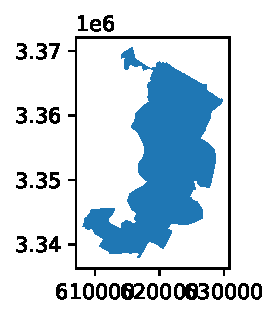
\includegraphics{spatial_2_files/figure-beamer/cell-6-output-1.pdf}

Discussion question: Why isn't it enough to just to \texttt{head()}?
\end{frame}

\begin{frame}[fragile]{Geopandas summary}
\phantomsection\label{geopandas-summary}
\begin{itemize}
\tightlist
\item
  \texttt{GeoDataFrame} and \texttt{GeoSeries} are the counterparts of
  \texttt{pandas.DataFrame} and \texttt{pandas.Series}
\item
  \texttt{.shp} and \texttt{.gpkg} are two ways of storing geo data
\item
  Always plot your map before you do anything else
\end{itemize}
\end{frame}

\section{Geometries in geopandas
(6.2)}\label{geometries-in-geopandas-6.2}

\begin{frame}[fragile]{geometries: roadmap}
\phantomsection\label{geometries-roadmap}
\begin{itemize}
\tightlist
\item
  methods applied to \texttt{GeoSeries}
\item
  my first choropleth
\end{itemize}
\end{frame}

\begin{frame}[fragile]{\texttt{GeoSeries}}
\phantomsection\label{geoseries}
\begin{Shaded}
\begin{Highlighting}[]
\BuiltInTok{type}\NormalTok{(data[}\StringTok{"geometry"}\NormalTok{])}
\end{Highlighting}
\end{Shaded}

\begin{verbatim}
geopandas.geoseries.GeoSeries
\end{verbatim}
\end{frame}

\begin{frame}[fragile]{\texttt{head()}}
\phantomsection\label{head}
\scriptsize

\begin{Shaded}
\begin{Highlighting}[]
\NormalTok{data[}\StringTok{"geometry"}\NormalTok{].head()}
\end{Highlighting}
\end{Shaded}

\begin{verbatim}
0    POLYGON ((615643.487 3338728.496, 615645.477 3...
1    POLYGON ((618576.586 3359381.053, 618614.33 33...
2    POLYGON ((619200.163 3341784.654, 619270.849 3...
3    POLYGON ((621623.757 3350508.165, 621656.294 3...
4    POLYGON ((621630.247 3345130.744, 621717.926 3...
Name: geometry, dtype: geometry
\end{verbatim}

\normalsize
\end{frame}

\begin{frame}[fragile]{calculate area (in square meters)}
\phantomsection\label{calculate-area-in-square-meters}
\begin{Shaded}
\begin{Highlighting}[]
\NormalTok{data[}\StringTok{"geometry"}\NormalTok{].area}
\end{Highlighting}
\end{Shaded}

\begin{verbatim}
0      4.029772e+06
1      1.532030e+06
2      3.960344e+06
3      2.181762e+06
4      2.431208e+06
           ...     
125    2.321182e+06
126    4.388407e+06
127    1.702764e+06
128    3.540893e+06
129    2.054702e+06
Length: 130, dtype: float64
\end{verbatim}
\end{frame}

\begin{frame}[fragile]{add column to data frame}
\phantomsection\label{add-column-to-data-frame}
\scriptsize

\begin{Shaded}
\begin{Highlighting}[]
\CommentTok{\#data.area is just a shorthand for data.geometry.area}
\NormalTok{data[}\StringTok{"area\_km2"}\NormalTok{] }\OperatorTok{=}\NormalTok{ data.area }\OperatorTok{/} \DecValTok{1000000}
\NormalTok{data[[}\StringTok{\textquotesingle{}tract\textquotesingle{}}\NormalTok{, }\StringTok{\textquotesingle{}area\_km2\textquotesingle{}}\NormalTok{, }\StringTok{\textquotesingle{}geometry\textquotesingle{}}\NormalTok{]].head()}
\end{Highlighting}
\end{Shaded}

\begin{longtable}[]{@{}llll@{}}
\toprule\noalign{}
& tract & area\_km2 & geometry \\
\midrule\noalign{}
\endhead
0 & 002422 & 4.029772 & POLYGON ((615643.487 3338728.496, 615645.477
3... \\
1 & 001751 & 1.532030 & POLYGON ((618576.586 3359381.053, 618614.33
33... \\
2 & 002411 & 3.960344 & POLYGON ((619200.163 3341784.654, 619270.849
3... \\
3 & 000401 & 2.181762 & POLYGON ((621623.757 3350508.165, 621656.294
3... \\
4 & 002313 & 2.431208 & POLYGON ((621630.247 3345130.744, 621717.926
3... \\
\bottomrule\noalign{}
\end{longtable}

\normalsize
\end{frame}

\begin{frame}[fragile]{my first choropleth}
\phantomsection\label{my-first-choropleth}
\begin{Shaded}
\begin{Highlighting}[]
\NormalTok{data.plot(column}\OperatorTok{=}\StringTok{"area\_km2"}\NormalTok{, legend}\OperatorTok{=}\VariableTok{True}\NormalTok{)}
\end{Highlighting}
\end{Shaded}

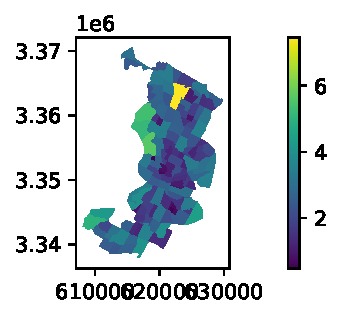
\includegraphics{spatial_2_files/figure-beamer/cell-11-output-1.pdf}

Discussion question -- why is this a nearly useless set of colors?
\end{frame}

\begin{frame}[fragile]{geometries: summary}
\phantomsection\label{geometries-summary}
\begin{itemize}
\tightlist
\item
  can do all the same operations on a \texttt{GeoSeries} that you would
  do on any other polygon, like \texttt{Area}
\item
  \texttt{data.plot(column="var")} draws a choropleth map with shading
  corresponding to the highlighted variable
\end{itemize}
\end{frame}

\section{Common geometric operations
(6.3)}\label{common-geometric-operations-6.3}

\begin{frame}{common geometric operations: roadmap}
\phantomsection\label{common-geometric-operations-roadmap}
\begin{itemize}
\tightlist
\item
  load and explore data
\item
  methods

  \begin{itemize}
  \tightlist
  \item
    centroid
  \item
    bounding box
  \item
    buffer
  \item
    dissolve
  \item
    spatial join
  \end{itemize}
\item
  do-pair-share
\end{itemize}
\end{frame}

\begin{frame}[fragile]{Austin, continued}
\phantomsection\label{austin-continued}
(The textbook uses a slightly different file here, unclear why to us.)

\begin{Shaded}
\begin{Highlighting}[]
\NormalTok{filepath }\OperatorTok{=} \StringTok{"data/austin\_pop\_density\_2019.gpkg"}
\NormalTok{data }\OperatorTok{=}\NormalTok{ gpd.read\_file(filepath)}
\end{Highlighting}
\end{Shaded}
\end{frame}

\begin{frame}[fragile]{explore the data I}
\phantomsection\label{explore-the-data-i}
\begin{Shaded}
\begin{Highlighting}[]
\NormalTok{data.head()}
\end{Highlighting}
\end{Shaded}

\begin{longtable}[]{@{}llllll@{}}
\toprule\noalign{}
& pop2019 & tract & area\_km2 & pop\_density\_km2 & geometry \\
\midrule\noalign{}
\endhead
0 & 6070.0 & 002422 & 4.029772 & 1506.288778 & MULTIPOLYGON
(((615643.488 3338728.496, 615645... \\
1 & 2203.0 & 001751 & 1.532030 & 1437.961394 & MULTIPOLYGON
(((618576.586 3359381.053, 618614... \\
2 & 7419.0 & 002411 & 3.960344 & 1873.322161 & MULTIPOLYGON
(((619200.163 3341784.654, 619270... \\
3 & 4229.0 & 000401 & 2.181762 & 1938.341859 & MULTIPOLYGON
(((621623.757 3350508.165, 621656... \\
4 & 4589.0 & 002313 & 2.431208 & 1887.538658 & MULTIPOLYGON
(((621630.247 3345130.744, 621717... \\
\bottomrule\noalign{}
\end{longtable}
\end{frame}

\begin{frame}[fragile]{explore the data II}
\phantomsection\label{explore-the-data-ii}
\begin{Shaded}
\begin{Highlighting}[]
\BuiltInTok{type}\NormalTok{(data[}\StringTok{"geometry"}\NormalTok{].values[}\DecValTok{0}\NormalTok{])}
\end{Highlighting}
\end{Shaded}

\begin{verbatim}
shapely.geometry.multipolygon.MultiPolygon
\end{verbatim}
\end{frame}

\begin{frame}[fragile]{explore the data III}
\phantomsection\label{explore-the-data-iii}
\begin{Shaded}
\begin{Highlighting}[]
\ImportTok{import}\NormalTok{ matplotlib.pyplot }\ImportTok{as}\NormalTok{ plt}
\NormalTok{data.plot(facecolor}\OperatorTok{=}\StringTok{"none"}\NormalTok{, linewidth}\OperatorTok{=}\FloatTok{0.2}\NormalTok{)}
\NormalTok{plt.axis(}\StringTok{"off"}\NormalTok{)}
\NormalTok{plt.show()}
\end{Highlighting}
\end{Shaded}

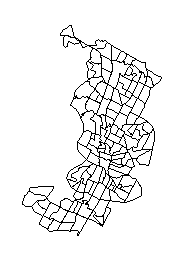
\includegraphics{spatial_2_files/figure-beamer/cell-15-output-1.pdf}

\begin{itemize}
\tightlist
\item
  Import \texttt{matplotlib.pyplot} to access additional plotting
  options (e.g., x and y labels, title)
\item
  We turn the axis off because the WKT is not informative
\end{itemize}
\end{frame}

\begin{frame}[fragile]{explore the data IV}
\phantomsection\label{explore-the-data-iv}
\begin{Shaded}
\begin{Highlighting}[]
\NormalTok{data.plot(column}\OperatorTok{=}\StringTok{"pop\_density\_km2"}\NormalTok{)}
\NormalTok{plt.axis(}\StringTok{"off"}\NormalTok{)}
\NormalTok{plt.show()}
\end{Highlighting}
\end{Shaded}

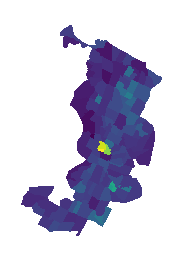
\includegraphics{spatial_2_files/figure-beamer/cell-16-output-1.pdf}

\begin{itemize}
\tightlist
\item
  \texttt{facecolor} (or \texttt{fc} or \texttt{color}) defines a
  uniform color across all geometries
\item
  whereas \texttt{columns} generates colors based on the underlying
  values
\end{itemize}
\end{frame}

\begin{frame}[fragile]{methods: centroid I}
\phantomsection\label{methods-centroid-i}
What it is: arithmetic mean position of all the points in a polygon

Sample use case: measuring distance between center of each multipolygon

\begin{Shaded}
\begin{Highlighting}[]
\NormalTok{data[}\StringTok{"geometry"}\NormalTok{].centroid.head()}
\end{Highlighting}
\end{Shaded}

\begin{verbatim}
0     POINT (616990.19 3339736.002)
1    POINT (619378.303 3359650.002)
2    POINT (620418.753 3342194.171)
3    POINT (622613.506 3351414.386)
4    POINT (622605.359 3343869.554)
dtype: geometry
\end{verbatim}
\end{frame}

\begin{frame}[fragile]{methods: centroid II}
\phantomsection\label{methods-centroid-ii}
\begin{Shaded}
\begin{Highlighting}[]
\NormalTok{data.centroid.plot(markersize}\OperatorTok{=}\DecValTok{1}\NormalTok{)}
\NormalTok{plt.axis(}\StringTok{"off"}\NormalTok{)}
\NormalTok{plt.show()}
\end{Highlighting}
\end{Shaded}

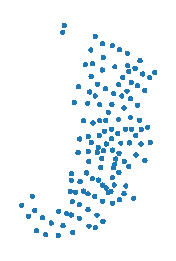
\includegraphics{spatial_2_files/figure-beamer/cell-18-output-1.pdf}
\end{frame}

\begin{frame}{centroid example outside polygon}
\phantomsection\label{centroid-example-outside-polygon}
\includegraphics[width=\textwidth,height=0.8\textheight]{pictures/census-usa-example_zoom19.png}

Source:
https://spatialanalysisonline.com/HTML/centroids\_and\_centers.htm
\end{frame}

\begin{frame}[fragile]{aside: change active geometry}
\phantomsection\label{aside-change-active-geometry}
\scriptsize

\begin{Shaded}
\begin{Highlighting}[]
\NormalTok{data[}\StringTok{"centroid"}\NormalTok{] }\OperatorTok{=}\NormalTok{ data.centroid}
\NormalTok{data.set\_geometry(}\StringTok{"centroid"}\NormalTok{)}
\NormalTok{data[[}\StringTok{\textquotesingle{}tract\textquotesingle{}}\NormalTok{, }\StringTok{\textquotesingle{}centroid\textquotesingle{}}\NormalTok{, }\StringTok{\textquotesingle{}geometry\textquotesingle{}}\NormalTok{]].head()}
\end{Highlighting}
\end{Shaded}

\begin{longtable}[]{@{}llll@{}}
\toprule\noalign{}
& tract & centroid & geometry \\
\midrule\noalign{}
\endhead
0 & 002422 & POINT (616990.19 3339736.002) & MULTIPOLYGON (((615643.488
3338728.496, 615645... \\
1 & 001751 & POINT (619378.303 3359650.002) & MULTIPOLYGON (((618576.586
3359381.053, 618614... \\
2 & 002411 & POINT (620418.753 3342194.171) & MULTIPOLYGON (((619200.163
3341784.654, 619270... \\
3 & 000401 & POINT (622613.506 3351414.386) & MULTIPOLYGON (((621623.757
3350508.165, 621656... \\
4 & 002313 & POINT (622605.359 3343869.554) & MULTIPOLYGON (((621630.247
3345130.744, 621717... \\
\bottomrule\noalign{}
\end{longtable}

\normalsize
\end{frame}

\begin{frame}{methods: bounding box definition}
\phantomsection\label{methods-bounding-box-definition}
What it is: the tightest possible rectangle around a shape, capturing
all of its points within this rectangle.

Sample use case: filtering a larger spatial dataset to subset of
interest
\end{frame}

\begin{frame}[fragile]{methods: bounding box for each polygon I}
\phantomsection\label{methods-bounding-box-for-each-polygon-i}
\begin{Shaded}
\begin{Highlighting}[]
\NormalTok{data.envelope.head()}
\end{Highlighting}
\end{Shaded}

\begin{verbatim}
0    POLYGON ((615643.488 3337909.895, 618358.033 3...
1    POLYGON ((618529.497 3358797, 620192.632 33587...
2    POLYGON ((619198.456 3340875.421, 621733.88 33...
3    POLYGON ((621599.087 3350329.32, 623714.365 33...
4    POLYGON ((621630.247 3343015.679, 624133.189 3...
dtype: geometry
\end{verbatim}
\end{frame}

\begin{frame}[fragile]{methods: bounding box for each polygon II}
\phantomsection\label{methods-bounding-box-for-each-polygon-ii}
\begin{Shaded}
\begin{Highlighting}[]
\NormalTok{data.envelope.plot()}
\end{Highlighting}
\end{Shaded}

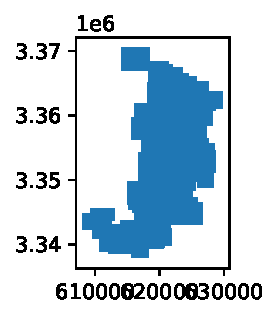
\includegraphics{spatial_2_files/figure-beamer/cell-21-output-1.pdf}
\end{frame}

\begin{frame}[fragile]{methods: bounding box for whole data I}
\phantomsection\label{methods-bounding-box-for-whole-data-i}
\scriptsize

\begin{Shaded}
\begin{Highlighting}[]
\NormalTok{data.total\_bounds}
\end{Highlighting}
\end{Shaded}

\begin{verbatim}
array([ 608125.39429998, 3337909.89499998,  629828.38850021,
       3370513.68260002])
\end{verbatim}

\normalsize
\end{frame}

\begin{frame}[fragile]{methods: bounding box for whole data II}
\phantomsection\label{methods-bounding-box-for-whole-data-ii}
Flashback to section 6.1

\begin{Shaded}
\begin{Highlighting}[]
\ImportTok{from}\NormalTok{ shapely }\ImportTok{import}\NormalTok{ Point, Polygon}
\NormalTok{point1 }\OperatorTok{=}\NormalTok{ Point(data.total\_bounds[}\DecValTok{0}\NormalTok{], data.total\_bounds[}\DecValTok{1}\NormalTok{])}
\NormalTok{point2 }\OperatorTok{=}\NormalTok{ Point(data.total\_bounds[}\DecValTok{2}\NormalTok{], data.total\_bounds[}\DecValTok{1}\NormalTok{])}
\NormalTok{point3 }\OperatorTok{=}\NormalTok{ Point(data.total\_bounds[}\DecValTok{2}\NormalTok{], data.total\_bounds[}\DecValTok{3}\NormalTok{])}
\NormalTok{point4 }\OperatorTok{=}\NormalTok{ Point(data.total\_bounds[}\DecValTok{0}\NormalTok{], data.total\_bounds[}\DecValTok{3}\NormalTok{])}
\NormalTok{poly }\OperatorTok{=}\NormalTok{ Polygon([point1, point2, point3, point4])}
\CommentTok{\#poly}
\end{Highlighting}
\end{Shaded}

\begin{itemize}
\tightlist
\item
  \emph{Note}: the order in which you put these points together matters,
  and you'll get all sorts of interesting shapes with different orders!
\end{itemize}
\end{frame}

\begin{frame}{methods: buffer I}
\phantomsection\label{methods-buffer-i}
What it is: shape representing all points that are less than a certain
distance from the original shape

Sample use cases:

\begin{itemize}
\tightlist
\item
  how many stores or parks near a neighborhood
\item
  geometries that don't line up well (e.g.~coasts)
\item
  selecting nearby geometries
\end{itemize}
\end{frame}

\begin{frame}[fragile]{methods: buffer II}
\phantomsection\label{methods-buffer-ii}
\begin{Shaded}
\begin{Highlighting}[]
\NormalTok{data.}\BuiltInTok{buffer}\NormalTok{(}\DecValTok{1000}\NormalTok{).plot(edgecolor}\OperatorTok{=}\StringTok{"white"}\NormalTok{) }\CommentTok{\#1000 meters}
\NormalTok{plt.axis(}\StringTok{"off"}\NormalTok{)}
\NormalTok{plt.show()}
\end{Highlighting}
\end{Shaded}


\includegraphics{spatial_2_files/figure-beamer/cell-24-output-1.pdf}
\end{frame}

\begin{frame}[fragile]{methods: dissolve I}
\phantomsection\label{methods-dissolve-i}
What it is: combining geometries into coarser spatial units based on
some attributes.

Sample use case: construct the geometries that you want to serve with
public transit

\begin{Shaded}
\begin{Highlighting}[]
\CommentTok{\# Create a new column and add a constant value}
\NormalTok{data[}\StringTok{"dense"}\NormalTok{] }\OperatorTok{=} \DecValTok{0}

\CommentTok{\# Filter rows with above average pop density and update the column dense}
\NormalTok{data.loc[data[}\StringTok{"pop\_density\_km2"}\NormalTok{] }\OperatorTok{\textgreater{}}\NormalTok{ data[}\StringTok{"pop\_density\_km2"}\NormalTok{].mean(), }\StringTok{"dense"}\NormalTok{] }\OperatorTok{=} \DecValTok{1}
\NormalTok{data.dense.value\_counts()}
\end{Highlighting}
\end{Shaded}

\begin{verbatim}
dense
0    86
1    44
Name: count, dtype: int64
\end{verbatim}
\end{frame}

\begin{frame}[fragile]{methods: dissolve II}
\phantomsection\label{methods-dissolve-ii}
\scriptsize

\begin{Shaded}
\begin{Highlighting}[]
\NormalTok{dissolved }\OperatorTok{=}\NormalTok{ data[[}\StringTok{"pop2019"}\NormalTok{, }\StringTok{"area\_km2"}\NormalTok{, }\StringTok{"dense"}\NormalTok{, }\StringTok{"geometry"}\NormalTok{]].dissolve(}
\NormalTok{    by}\OperatorTok{=}\StringTok{"dense"}\NormalTok{, aggfunc}\OperatorTok{=}\StringTok{"sum"}
\NormalTok{)}
\CommentTok{\#aggregation step set index to "dense", reset to default}
\NormalTok{dissolved }\OperatorTok{=}\NormalTok{ dissolved.reset\_index()}
\NormalTok{dissolved}
\end{Highlighting}
\end{Shaded}

\begin{longtable}[]{@{}lllll@{}}
\toprule\noalign{}
& dense & geometry & pop2019 & area\_km2 \\
\midrule\noalign{}
\endhead
0 & 0 & MULTIPOLYGON (((614108.23 3339640.551, 614288.... & 368992.0 &
231.131494 \\
1 & 1 & MULTIPOLYGON (((612263.531 3338931.8, 612265.2... & 242943.0 &
71.234570 \\
\bottomrule\noalign{}
\end{longtable}

\normalsize

\begin{itemize}
\tightlist
\item
  Aggregating alters the way the data is indexed and makes the grouping
  variable the index
\item
  We need to reset it in order to plot, since some plotting libraries
  expect data to be indexed in a specific way
\end{itemize}
\end{frame}

\begin{frame}[fragile]{methods: dissolve III}
\phantomsection\label{methods-dissolve-iii}
\begin{Shaded}
\begin{Highlighting}[]
\NormalTok{dissolved.plot(column}\OperatorTok{=}\StringTok{"dense"}\NormalTok{)}
\NormalTok{plt.axis(}\StringTok{"off"}\NormalTok{)}
\NormalTok{plt.show()}
\end{Highlighting}
\end{Shaded}

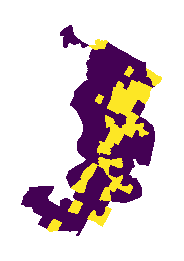
\includegraphics{spatial_2_files/figure-beamer/cell-27-output-1.pdf}

Discussion Question: What can we do to improve this map?
\end{frame}

\begin{frame}[fragile]{methods: spatial join}
\phantomsection\label{methods-spatial-join}
Spatial join: find the closest neighbor.

\begin{Shaded}
\begin{Highlighting}[]
\NormalTok{data\_for\_join }\OperatorTok{=}\NormalTok{ data[[}\StringTok{"tract"}\NormalTok{, }\StringTok{"geometry"}\NormalTok{]]}
\BuiltInTok{print}\NormalTok{(}\StringTok{"N tracts "} \OperatorTok{+} \BuiltInTok{str}\NormalTok{(}\BuiltInTok{len}\NormalTok{(data\_for\_join)))}
\NormalTok{join\_to\_self }\OperatorTok{=}\NormalTok{ gpd.sjoin\_nearest(}
\NormalTok{    data\_for\_join,  }\CommentTok{\#left df}
\NormalTok{    data\_for\_join, }\CommentTok{\#right df}
\NormalTok{    how}\OperatorTok{=}\StringTok{\textquotesingle{}inner\textquotesingle{}}\NormalTok{, }
\NormalTok{    distance\_col}\OperatorTok{=}\StringTok{"distance"}
\NormalTok{)}
\end{Highlighting}
\end{Shaded}

\begin{verbatim}
N tracts 130
\end{verbatim}

(Contrived) example: Join every Austin tract to its closest neighbor or
neighbors. How many tracts should we expect to get?
\end{frame}

\begin{frame}[fragile]{methods: spatial join II}
\phantomsection\label{methods-spatial-join-ii}
\begin{Shaded}
\begin{Highlighting}[]
\BuiltInTok{print}\NormalTok{(}\StringTok{"N tracts w closest neighbor "} \OperatorTok{+} 
    \BuiltInTok{str}\NormalTok{(}\BuiltInTok{len}\NormalTok{(join\_to\_self)))}
\NormalTok{join\_to\_self[[}\StringTok{\textquotesingle{}tract\_left\textquotesingle{}}\NormalTok{, }\StringTok{\textquotesingle{}tract\_right\textquotesingle{}}\NormalTok{, }\StringTok{\textquotesingle{}distance\textquotesingle{}}\NormalTok{]].head(}\DecValTok{4}\NormalTok{)}
\end{Highlighting}
\end{Shaded}

\begin{verbatim}
N tracts w closest neighbor 848
\end{verbatim}

\begin{longtable}[]{@{}llll@{}}
\toprule\noalign{}
& tract\_left & tract\_right & distance \\
\midrule\noalign{}
\endhead
0 & 002422 & 002423 & 0.0 \\
0 & 002422 & 002422 & 0.0 \\
0 & 002422 & 002424 & 0.0 \\
0 & 002422 & 002402 & 0.0 \\
\bottomrule\noalign{}
\end{longtable}
\end{frame}

\begin{frame}{common geometric operations: summary}
\phantomsection\label{common-geometric-operations-summary}
\begin{itemize}
\tightlist
\item
  methods

  \begin{itemize}
  \tightlist
  \item
    centroid computes arithmetic mean of points in the polygon
  \item
    bounding box expands polygon in a rectangle
  \item
    buffer expands polygon in every direction
  \item
    dissolve combines several polygons
  \item
    spatial join finds nearest neighbor
  \end{itemize}
\item
  do-pair-share
\end{itemize}
\end{frame}

\begin{frame}[fragile]{do pair share}
\phantomsection\label{do-pair-share}
Goal: Create and plot a 500m buffer zone around the dense areas in
Austin.

Steps

\begin{enumerate}
\tightlist
\item
  From the \texttt{dissolved} \texttt{GeoDataFrame}, get the polygon for
  the dense areas
\item
  Create a new geometry object called \texttt{geo}, which is the dense
  areas with a 500m buffer
\item
  \texttt{geo.plot()}
\end{enumerate}

\begin{Shaded}
\begin{Highlighting}[]
\NormalTok{austin }\OperatorTok{=}\NormalTok{ data.plot(color}\OperatorTok{=}\StringTok{"grey"}\NormalTok{)}
\NormalTok{geo }\OperatorTok{=}\NormalTok{ dissolved[dissolved[}\StringTok{"dense"}\NormalTok{] }\OperatorTok{==} \DecValTok{0}\NormalTok{].}\BuiltInTok{buffer}\NormalTok{(}\DecValTok{500}\NormalTok{)}
\NormalTok{geo.plot(ax}\OperatorTok{=}\NormalTok{austin, alpha}\OperatorTok{=}\FloatTok{0.4}\NormalTok{)}
\end{Highlighting}
\end{Shaded}

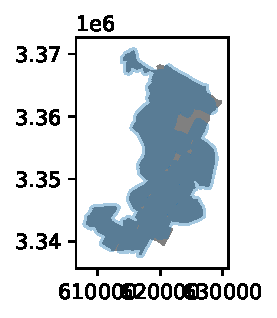
\includegraphics{spatial_2_files/figure-beamer/cell-30-output-1.pdf}

After you are done, here are some cosmetic suggestions:

\begin{itemize}
\tightlist
\item
  Start with a grey plot of all of the Austin boundaries:
  \texttt{austin\ =\ data.plot(color="grey")}
\item
  Make your buffer transparent
\item
  Putting it all together \texttt{geo.plot(ax\ =\ austin,\ alpha=0.5)}

  \begin{itemize}
  \tightlist
  \item
    This plots the \texttt{geo} object with 50\% transparency, on top of
    axes based on the \texttt{austin} object
  \end{itemize}
\end{itemize}
\end{frame}




\end{document}
